% TEMPLATE for Usenix papers, specifically to meet requirements of
%  USENIX '05
% originally a template for producing IEEE-format articles using LaTeX.
%   written by Matthew Ward, CS Department, Worcester Polytechnic Institute.
% adapted by David Beazley for his excellent SWIG paper in Proceedings,
%   Tcl 96
% turned into a smartass generic template by De Clarke, with thanks to
%   both the above pioneers
% use at your own risk.  Complaints to /dev/null.
% make it two column with no page numbering, default is 10 point

% Munged by Fred Douglis <douglis@research.att.com> 10/97 to separate
% the .sty file from the LaTeX source template, so that people can
% more easily include the .sty file into an existing document.  Also
% changed to more closely follow the style guidelines as represented
% by the Word sample file. 

% Note that since 2010, USENIX does not require endnotes. If you want
% foot of page notes, don't include the endnotes package in the 
% usepackage command, below.

\documentclass[letterpaper,twocolumn,10pt]{article}
\usepackage{usenix,epsfig,endnotes,hyperref,graphicx}
\begin{document}

%don't want date printed
\date{}

%make title bold and 14 pt font (Latex default is non-bold, 16 pt)
\title{\Large \bf Final Report: Jepsen Test for Apache Aurora and Apache Mesos}

\author{
{\rm Jin Fang}\\
Columbia University
\and
{\rm Jincheng Li}\\
Columbia University
\and
{\rm Lu Yang}\\
Columbia University
}
\maketitle

% Use the following at camera-ready time to suppress page numbers.
% Comment it out when you first submit the paper for review.
\thispagestyle{empty}


\subsection*{Abstract}
In this report we describe our work testing consistency properties of Apache Aurora and Apache Mesos under network partitions. We have set up a Jepsen test environment with Aurora and Mesos running in docker containers. We give our definition of the proper semantics of a scheduler service, and the design of corresponding procedures to test the behavior of Aurora with Jepsen under these definitions. The result shows that under the right configurations, the Aurora/Mesos system is robust under network partitions. 

\subsection*{Source Code}
The source code for this project can be found at \url{https://github.com/jchli/jepsen-aurora}.

\section{Introduction}
Mesos is a popular cluster management system. It is built using the same principles as the Linux kernel, only at a different level of abstraction. The Mesos kernel runs on every machine and provides applications (e.g., Hadoop, Spark, Kafka, Elastic Search) with API’s for resource management and scheduling across entire datacenter and cloud environments.~\cite{Mesos} The software enables resource sharing in a fine-grained manner, improving cluster utilization. Aurora is a service scheduler that runs on top of Mesos, enabling you to run long-running services that take advantage of Mesos’ scalability, fault-tolerance, and resource isolation~\cite{Aurora}.

We would like to investigate the correctness of the Aurora + Mesos system, which will be explained in more detail in section 4, with Jepsen, an open-source tool built for testing distributed systems. 

Mesos was first presented in 2009. This newly developed system is increasingly adopted recently by many companies such as Apple (Siri), Netflix, Twitter and Bloomberg. This rapidly increasing usage inspired us to test its capability of recovering from network partition, which is a large factor of distributed system performance.

\section{Related Work}
Aphyr, the author of  Jepsen, has conducted similar tests on the Chronos scheduler~\cite{Chronos}. Chronos is designed as a replacement for \verb|cron|. It is a distributed and fault-tolerant scheduler that runs on top of Apache Mesos that can be used for job orchestration. It supports custom Mesos executors as well as the default command executor. 

Our test for Aurora borrows heavily from ideas used in the Chronos test, so here we elaborate on the design of the Chronos test, its definition of semantics of a scheduler, and its results.

\subsection{Test Design}
The test setup is exemplary of most Jepsen tests: the cluster consists of 5 distinct nodes (labeled as n1 through n5), each running several different processes. For this particular test, Zookeeper runs across all 5 nodes. Mesos masters run on n1, n2, n3, while Mesos slaves run on n4 and n5. Finally, Chronos runs across all 5 nodes. And Chronos and Mesos depend on Zookeeper for Mesos to communicate with each other.

Next, job generation is done with a stateful generator which emits jobs with a unique integer \verb|:name|, a \verb|:start| time, a repetition \verb|:count|, a run \verb|:duration|, an \verb|:epsilon| window allowing jobs to run slightly late, and finally, an \verb|:interval| between the start of each window. This may seem like a complex way to generate tasks. It is designed to issue a variety of jobs with different configurations, and also to account for the behavior of Chronos. For example, Chronos takes a few seconds to spin up a task, which means that tasks often run a bit later than scheduled, hence the \verb|:epsilon| parameter. We want to ensure that the run begins somewhere between the target time t and t + epsilon –- but allow tasks to complete at their leisure. Also, each job we run consists of single tasks repeated multiple times, as specified by \verb|:count|. This allows us to observe how a job runs as network partitions are introduced.

Jobs behave in a simple way: they open a new file and write their job ID and current time, sleep for some duration, then, to indicate successful completion, write the current time again to the same file. This allows for reconstruction of the set of all runs by parsing the files from all nodes. Runs are considered complete if and only if they wrote a final timestamp. In this particular test, all node clocks are perfectly synchronized, so it is okay to union times from each node without correction.

With this basic infrastructure set up, the test proceeds as follows: The generator emits add-job operations with a 30 second delay between each, randomly staggered by up to 30 seconds. Meanwhile, the special nemesis process cycles between creating and resolving failures every 200 seconds. This phase proceeds for a few seconds, after which the nemesis resolves any ongoing failures and allows the system to stabilize. Finally, a single client reads the results of all runs.

In order to evaluate the results, a checker is implemented to examine the history of add-job and read operations. First of all, for each run we check whether it has a completion time indicating successful execution. Then, check whether the actual start time is within the expected time span. These two combined together indicate whether Chronos is doing what is expected.

\subsection{Semantics}
In the Chronos test, the correctness of the scheduler is defined as ``tasks run on time''. Intuitively this serves as a good measure of whether a scheduler is behaving as desired. Concretely, a job has a schedule which specifies the points in time when its tasks should be run, and the scheduler is correct if and only if it executes these tasks according to their schedules.

Since this is a distributed, fault-tolerant system, we expect there to be failures and re-runs of the same job. Thus we allow tasks to start running within a short window of time, which is specified by the \verb|:epsilon| parameter. If all tasks within a job run within their respective window of \verb|[:start, :start + :epsilon]|, then we consider the job requirement to be satisfied.

\subsection{Results}
As tested under Jepsen, Chronos hard-crashes in response to a network partition. Its recovery behavior is also highly dependent on Mesos performance in a network partition. Unfortunately, Mesos crashes all the time during network partitions, and this “fail-fast” philosophy may play out differently depending on what Mesos components you’re working with~\cite{Chronos}.

If you schedule jobs with intervals that are too frequent - even if they don’t overlap - Chronos can fail to run jobs on time, because the scheduler loop can not handle granularity finer than a certain threshold. Lowering the scheduler horizon allows Chronos to satisfy all executions for intervals around 30 seconds – so long as no network failures occur~\cite{Chronos}.

However, if the network does fail (for instance, if a partition cleanly isolates two nodes from the other three), Chronos will fail to run any jobs–even after the network recovers. As shown is Fig.1
\begin{figure}
\centering
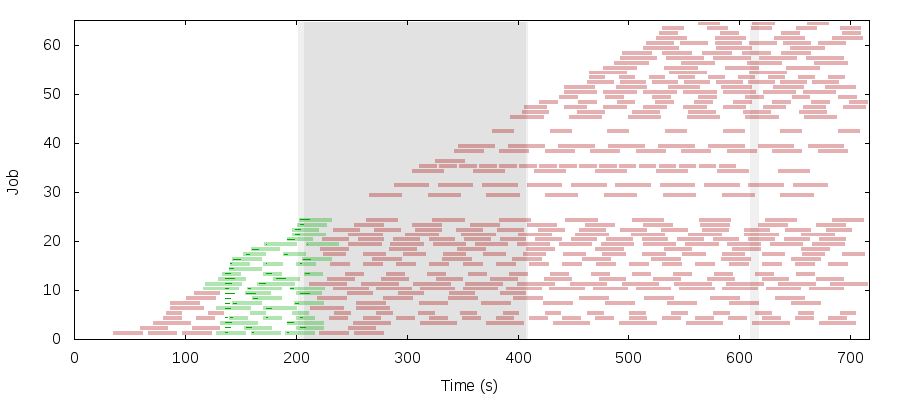
\includegraphics[width=3in]{chronos1}
\caption{Chronos recovery result1}
\label{fig:my_label}
\end{figure}

Fig.1 shows targets and runs for each job over time. Targets are thick bars, and runs are narrow, darker bars. Green targets are satisfied by a run beginning in their time window, and red targets show where a task without a completion time which indicates a failure. The Mesos master dies at the start of the test and no jobs run~\cite{Chronos}.

The gray region shows the duration of a network partition isolating [n2 n3] from [n1 n4 n5]. Chronos stops accepting new jobs for about a minute just after the partition, then recovers. ZK can continue running in the [n1 n4 n5] component, as can Chronos, but Mesos, to preserve a majority of its nodes [n1 n2 n3], can only allow a leading master in [n2 n3]. Isolating Chronos from the Mesos master prevents job execution during the partition–hence every target during the partition is red~\cite{Chronos}.

It illustrates the fragility of a system with three distinct quorums, all of which must be available and connected to one another, but there will always be certain classes of network failure that can break a distributed scheduler. What one might not expect, however, is that Chronos never recovers when the network heals. It continues accepting new jobs, but won’t run any jobs at all for the remainder of the test – every target is red even after the network heals. This behavior persists even when we give Chronos 1500+ seconds to recover~\cite{Chronos}. As shown in Fig.2

\begin{figure}
\centering
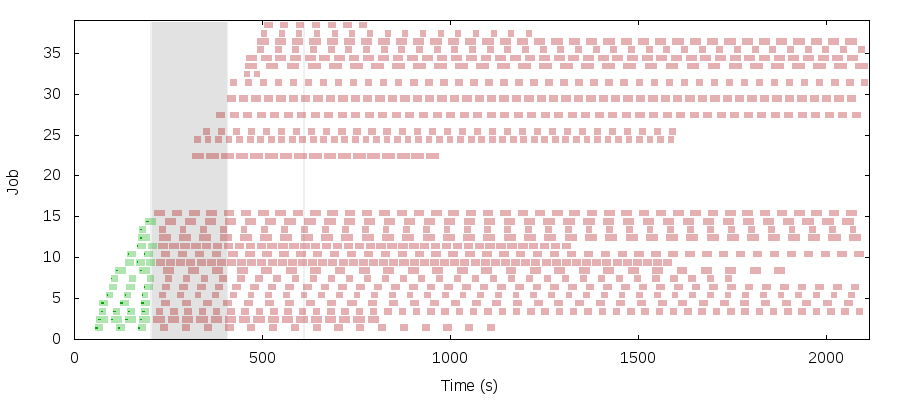
\includegraphics[width=3in]{chronos2}
\caption{Chronos recovery result2}
\label{fig:my_label}
\end{figure}

It turns out to be that after Chronos fails over, it registers with Mesos as an entirely new framework instead of re-registering. Mesos assumes the original Chronos framework still owns every resource in the cluster, and refuses to offer resources to the new Chronos leader. The first leader consume all resources when it only needed a small fraction of them~\cite{Chronos}.

As a workaround, the Chronos team recommended setting \verb|offer_timeout| to allow Mesos to reclaim resources from the misbehaving Chronos framework. They also recommend automatically restarting both Chronos and Mesos processes - both can recover from \emph{some} kinds of partitions but others cause them to crash~\cite{Chronos}.

\begin{figure}
\centering
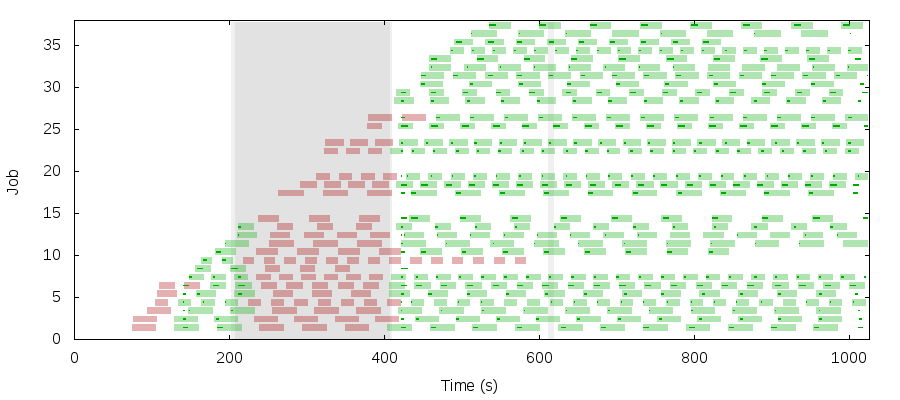
\includegraphics[width=3in]{chronos3}
\caption{Chronos recovery result3}
\label{fig:my_label}
\end{figure}
With these changes in place, Mesos may be able to recover some jobs but not others. Just after the partition resolves, it runs most jobs outside their target times~\cite{Chronos}. As shown in Fig.3

\section{System Setup}
Aurora relies on Mesos, which has two flavors of nodes: master nodes, and slave nodes. The master nodes themselves form a cluster with one leader and several followers, and this master cluster is coordinated with Zookeeper.

Mesos slaves connect to masters and offer resources like CPU, disk, and memory. Masters take these offers and make decisions about resource allocation using scheduling frameworks like Aurora.[1] Those decisions are sent to slaves, which actually run tasks on their respective nodes. Masters form a replicated state machine with a persistent log. Both masters and slaves rely on Zookeeper for coordination and discovery. Zookeeper is also used as a replicated persistent log~\cite{Aurora}. 

In our tests, we set up 5 docker containers to run Aurora, Mesos and Zookeeper instances. All five nodes run one instance of each of the three systems. Nodes $n1, n2,n3$ run Mesos master instances, while nodes $n4, n5$ run Mesos slave instances. The system architecture is shown below:\\
\begin{figure}
\centering
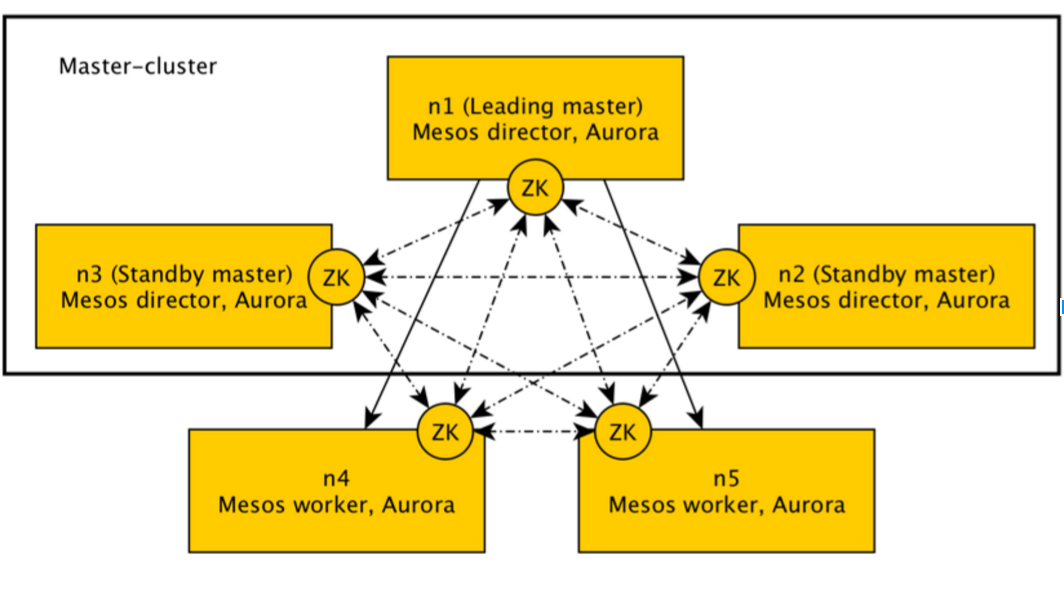
\includegraphics[width=3in]{systemSetup}
\caption{System Setup}
\label{fig:my_label}
\end{figure}

\section{Semantics}
In our analysis, the definition for the semantics of Aurora is similar to the one used for Chronos, that tasks run on time. And in a real-time environment, there will again be some small window of time during which the job should run. So a more practical measurement is that task should start running within \verb|[t, t+epsilon]|, where \verb|epsilon| is a small window of time.  

We have also considered an alternative perspective on the semantics of a scheduler. We could define the correctness of a scheduler to be the master’s view of available resources in the system. However, this definition brings with it implementation difficulties. For example, resources become available in real time, and it is hard to pinpoint a timestamp and ask simultaneously what the master's view of available resources is, and also what the actual pool of available resources is. This makes it difficult to verify if master has a correct view. Given that we have not figured out a way to take a snapshot of master and slaves’ view of available resources, we decided not to adopt this definition.

\section{Implementation Details}
This section details how we generate jobs, send them to Aurora, create network partitions and obtain results from nodes in the cluster.

\subsection{Deployment}
We start from five clean docker containers. In order to run Mesos and Aurora on them, we wrote bash scripts and Clojure code to install Mesos, Zookeeper, Aurora, and other necessary dependencies such as Java 8. The bash script to install Aurora is shown below:

\begin{verbatim}
#!/bin/bash

# check if aurora is already installed first
if [[ ! -e $AURORA_DIR ]]; then
    echo "installing aurora..."
    
    # add repo servers, certificates
    ...
    
    # install java 8
    apt-get install -y "oracle-java8.."

    # get aurora binary
    curl -L $AURORA_ZIP_LINK -o $AURORA_ZIP
    unzip -n $AURORA_ZIP -d "/usr/local"
    export PATH=$AURORA_DIR/bin:$PATH

    # Add Log output parameter
    mesos-log initialize --path=$AURORA_DIR/db

    echo "done"
fi

# install mesos egg and build thermos
if [[ ! -e "/aurora" ]]; then
    cd /
    apt-get update
    apt-get -y install gcc bison \
        curl git libapr1-dev \
        libcurl4-nss-dev libsasl2-dev \
        libsvn-dev python-dev zookeeperd
        
    git clone https://.../aurora.git
    pushd aurora
    
    mkdir -p third_party
    pushd third_party
    wget -c https://...-${MESOS_VERSION}.egg
    popd

    $deb=mesos_${MESOS_VERSION}-...deb
    wget -c http://.../$deb
    dpkg --install $deb
    
    ./pants binary ...:thermos_executor
    ./pants binary ...:thermos_runner
    
    # Package runner within executor.
    .../embed_runner_in_executor.py
    
    chmod +x .../thermos_executor.pex
    popd
fi
\end{verbatim}
For setting up Mesos and Zookeeper, we mostly stay the same with the Chronos test, which simply fetches sources from the Mesosphere repository and install them on cluster nodes.

\subsection{Job Generator}
The following bash script defines a task within a job: record the start time, sleep for a certain duration and record the end time. 
\begin{verbatim}
#!/bin/bash
…...
LOG=\$(mktemp -p " $JOB_RESULT_DIR "); " \
echo \"" $JOBNAME "\" >> $LOG; " \
    "date -u -Ins >> $LOG; " \
    "sleep " $DURATION "; " \
    "date -u -Ins >> $LOG;" \

…...
$AURORA_CLIENT job create
testcluster/www-data/devel/$JOBNAME 
$JOBCONFIG

\end{verbatim}

This is again similar to task definitions used in the Chronos test. These tasks do not take up a lot of slave resources (which turns out to be scarce with our setup, as will be explained), and enable us to analyze the results easily. The existence of a completion timestamp indicates a finished task, and we can use this data to determine whether a job has been correctly scheduled and executed.

\subsection{Client}
Aurora scheduler and Chronos scheduler use different methods to post a job. Chronos uses HTTP request with a specialized format to send a job. Aurora uses a client in the form of a PEX executable file to issue jobs, and a job configuration language to specify the job you want to post.

Thus we use a client to keep posting the jobs created by the job generator (in bash format), and we configure our jobs with the Aurora-specified job configuration language, as shown below:

\begin{verbatim}
TEMPCONFIG=$TEMPJOB.aurora
echo "
# run the script
$NAME = Process(
  name = '$NAME',
  min_duration = $(($DURATION * 2)),
  cmdline = '$(cat ${TEMPJOB})')

# describe the task
$TASKNAME = SequentialTask(
  processes = [$NAME],
  resources = Resources(cpu = 0.01,
  ram = 1*MB, disk=1*MB))

jobs = [
  Service(cluster = 'testcluster',
          environment = 'devel',
          role = 'www-data',
          name = '$NAME',
          task = $TASKNAME)
]" > $TEMPCONFIG

$AURORA_CLIENT job create testcluster/
www-data/devel/$NAME $TEMPCONFIG
\end{verbatim}

\subsection{Nemesis}
The nemesis in our test randomly partitions the cluster into two separate halves. Also, after the partition persists for some time, the nemesis is responsible for healing the partition and resurrecting any failed nodes. Since there are five nodes, we partition the nodes into a 2-node half and a 3-node half. All connections across these two halves are disabled, while nodes within each half can communicate as usual. We resurrect failed nodes because Aurora and Mesos services can stop after a timeout threshold when they cannot find a leader node. 

\subsection{Test Setup}
Our Aurora client runs on the parent node (where we run Jepsen). The Jepsen library forks the job generator process into 5 different threads, one for each node, so that the 5 threads concurrently issue jobs to the cluster. A job in our test has four parameters: name, start, duration, epsilon. Name is important for grouping together different runs of tasks that belong to the same job. Epsilon defines the window of time when the job is allowed to start. Start and duration simply define the characteristics of the job.


The following snippet of Clojure code shows what we use to add a new job.
\begin{verbatim}
(defn add-job!
  "Submits a new job to Aurora"
  [node job]
  (shell/sh "/jepsen/jepsen-aurora/
  scripts/add-job.sh" 
          (str (:name job))
          (str (:duration job))))
\end{verbatim}

Unlike the Chronos test, where every target task is run a finite number of times separated by variable intervals, we run every task as a service for Aurora, and every task will be run exactly every minute. Thus every job will run from the moment it starts to the end of the Jepsen test. This is not the ideal setup we would like, but unfortunately Aurora does not allow a task to be repeated, say, every 5 seconds. A regular task, when specified as something that should be repeated, will start immediately after it completes. Only tasks in the form of a cron job can be re-executed periodically with intervals, but cron jobs have intervals at the granularity of a minute. Thus we decided to use cron jobs to implement the test, and we set the interval between tasks to exactly one minute to speed up our tests. 

\begin{figure}
\centering
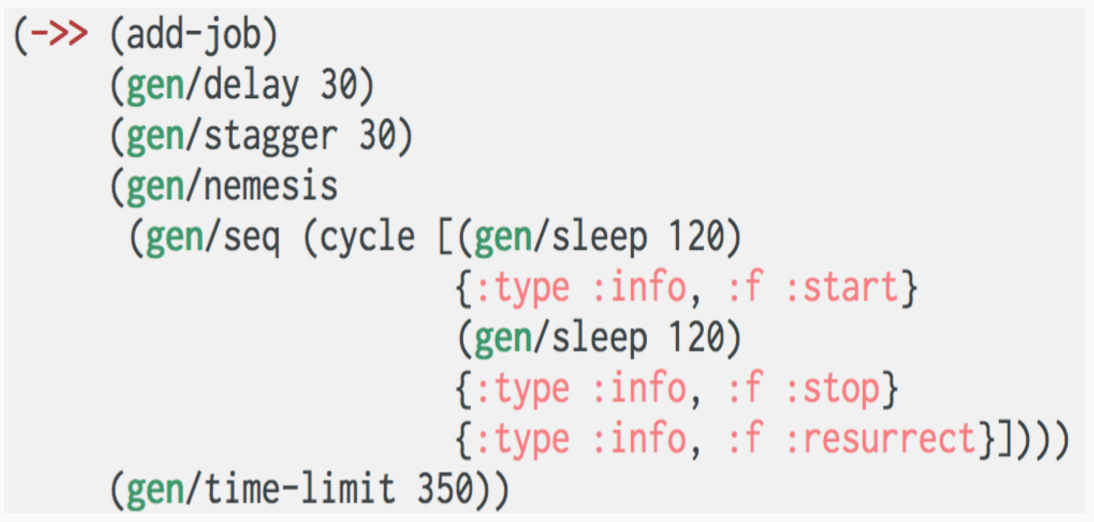
\includegraphics[width=3in]{jobGenerator}
\caption{Job Generator}
\label{fig:my_label}
\end{figure}

\section{Results}
We copy results from each node onto the parent node after Jepsen test finishes. We then analyze the results in exactly the same way as the Chronos scheduler test.


\begin{figure}
\centering
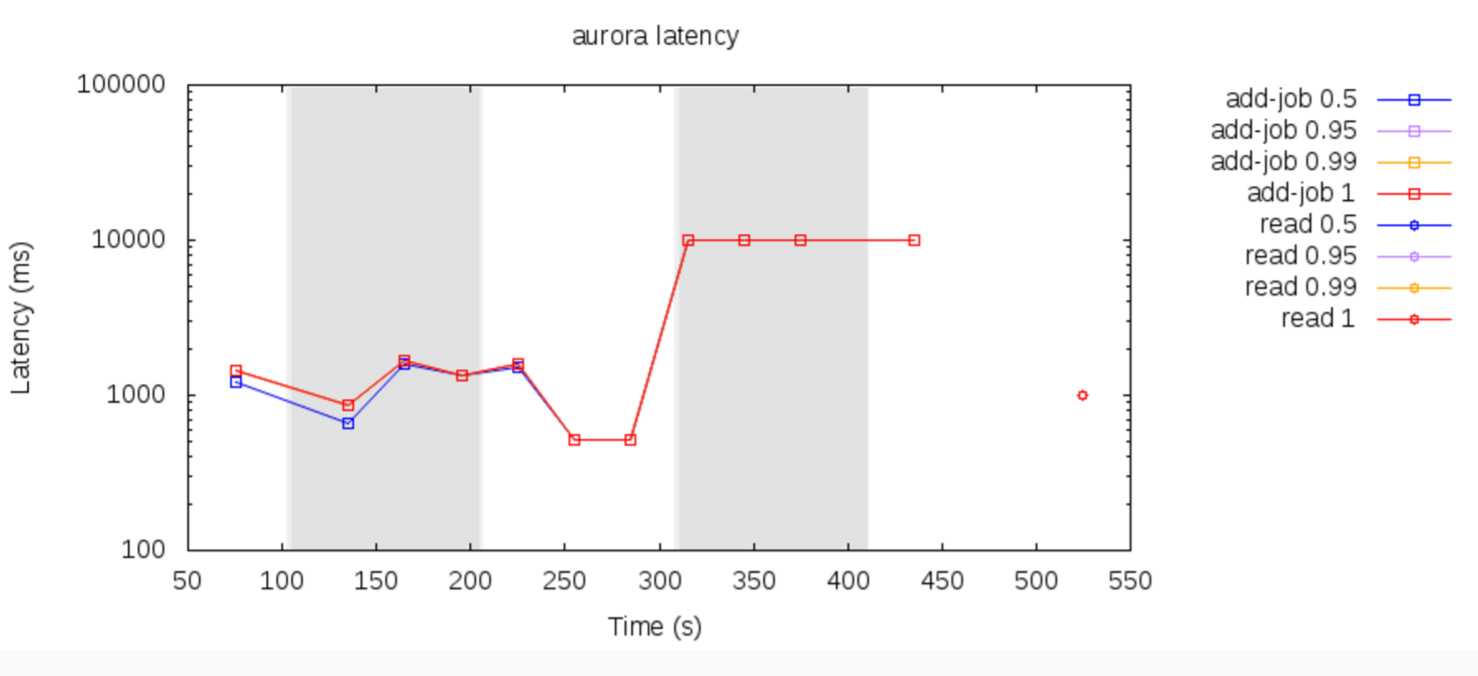
\includegraphics[width=3in]{latency}
\caption{Latency}
\label{fig:my_label}
\end{figure}

\begin{figure}
\centering
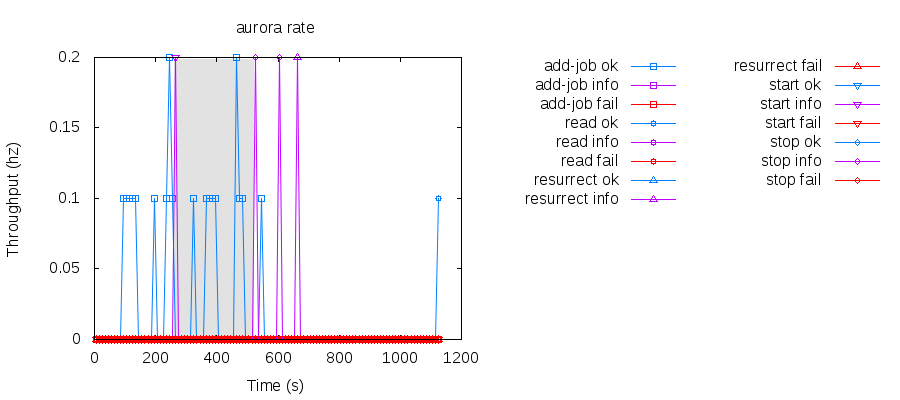
\includegraphics[width=3in]{rate}
\caption{Rate}
\label{fig:my_label}
\end{figure}

\begin{figure}
\centering
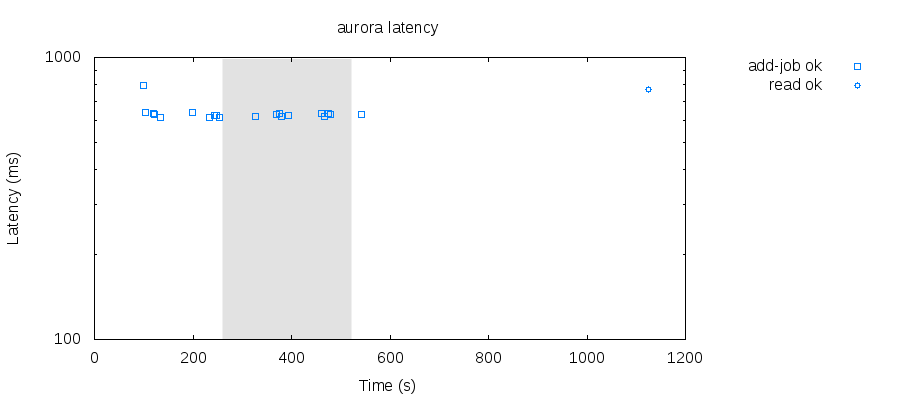
\includegraphics[width=3in]{latency-raw}
\caption{Raw latency}
\label{fig:my_label}
\end{figure}

\begin{figure}
\centering
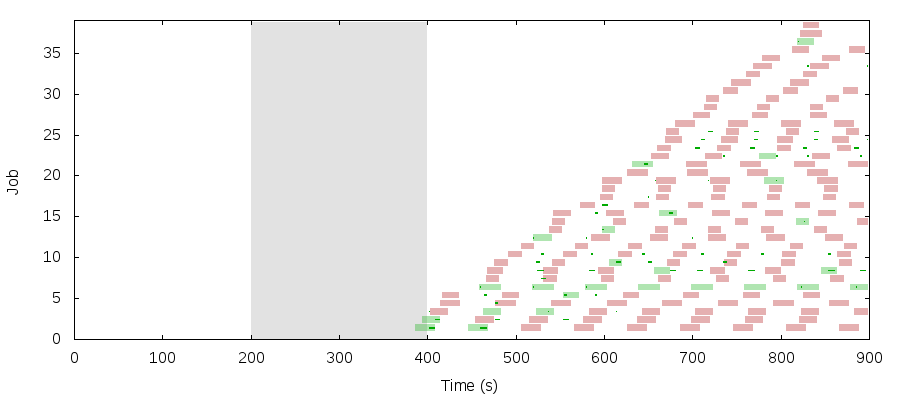
\includegraphics[width=3in]{aurora}
\caption{Result without partition}
\label{fig:my_label}
\end{figure}



\begin{figure}
\centering
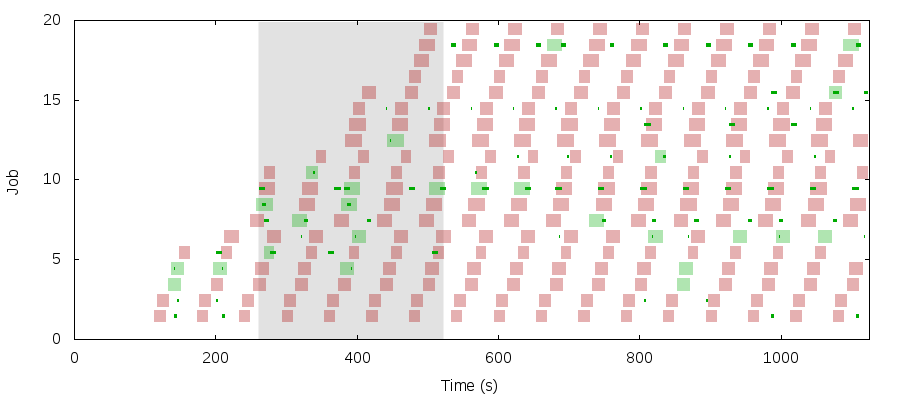
\includegraphics[width=3in]{aurora-partition}
\caption{Result with partition}
\label{fig:my_label}
\end{figure}

\subsection{Logs}
Below is shown an example of our log file which records the standard output of our tests. It consists of a sequence of add-job operations, definitions of the jobs, whether they were successfully added or timed-out, nemesis tags indicating when the network was partitioned and healed, and finally the list of results from tasks.

\begin{verbatim}
0	:invoke	:add-job	{:name 2, :start #object
[org.joda.time.DateTime 0xd856440
"2015-12-11T04:13:13.210Z"], 
:count 300, :duration 1, :epsilon 14}
0	:ok	:add-job	{:name 2, :start
#object[org.joda.time.DateTime 0xd856440
"2015-12-11T04:13:13.210Z"], 
:count 300, :duration 1, :epsilon 14}
...

:nemesis	:info	:start	
"Cut off {:n4 #{:n3 :n2 :n5}, :n1 #{:n3 :n2
:n5}, 
:n3 #{:n4 :n1}, :n2 #{:n4 :n1}, :n5 #{:n4
:n1}}"
3	:invoke	:add-job	
{:name 12, 
:start #object[org.joda.time.DateTime
0x7d9f7d23 "2015-12-11T04:15:01.818Z"], 
:count 300, :duration 9, :epsilon 19}
0	:info	:add-job	:timed-out

...

:nemesis	:info	:stop	nil
:nemesis	:info	:resurrect	nil

...


6	:ok	:read	({:node "n4", :name 1, 
:start #object[org.joda.time.DateTime 
0x14c63e9f "2015-12-19T01:08:07.167Z"], 
:end #object[org.joda.time.DateTime 
0x39d75008 "2015-12-19T01:08:07.168Z"]} 
{:node "n4", :name 5, :start ..., 
:end ...} {:node "n4", :name 2, :start ..., 
:end ...} ...)

\end{verbatim}

\subsection{Analysis}
Fig.7 and Fig. 8 show the status of operations in our test such as starting the cluster, adding a job, reading results. We can see that there is no failure adding jobs to the clusters. Note that our client is aware of all five nodes running the Aurora scheduler, whether they are in standby mode or serving as the active scheduler for Mesos. Thus at least in terms of interacting with the client and adding jobs, the Aurora scheduler is robust under network partitions. 

Fig. 9 and Fig. 10 show the behavior of Aurora with or without network partitions. We can see that mostly, there are tasks that succeed and fail in either scenario. Some tasks succeed most of the time. Some tasks succeed only a few times. Others simply never get to run. Note that although the figures show a lot of unmet targets (red rectangles), this only means that the tasks did not run on time. A lot of tasks ran as scheduled, but they were ran a bit too late. These are shown as dark-green rectangles on the plot.

Compared to the Chronos results this is very unexpected. We investigated why this is the case and attempted to fix it. By checking Mesos master logs, we discovered that during the runs, it kept prompting that there was not enough resource.

\begin{verbatim}
...
I1216 06:59:35.713598  4991 network.hpp:424]
ZooKeeper group memberships changed
I1216 06:59:35.720410  4993 detector.cpp:138] 
Detected a new leader: (id='1')
I1216 06:59:35.720448  4995 group.cpp:659]
Trying to get '/mesos/log_replicas/00000
00000'
in ZooKeeper
I1216 06:59:35.720604  4991 group.cpp:659]
Trying to get '/mesos/info_0000000001'
in ZooKeeper
I1216 06:59:35.722689  4991 detector.cpp:452] 
A new leading master (UPID=master@10.0.0.2
:5050)
is detected
I1216 06:59:35.722699  4987 network.hpp:466]
ZooKeeper group PIDs: { log-replica(1)
@10.0.0.2:
5050 }
I1216 06:59:35.722841  4991 master.cpp:1356]
The newly 
elected leader is master@10.0.0.2:
5050 with id 20151216-065935-33554442-
5050-4982
I1216 06:59:35.722904  4991 master.cpp:1369]
Elected as the leading master!
I1216 06:59:35.722939  4991 master.cpp:1187]
Recovering from registrar
I1216 06:59:35.723027  4984 registrar.
cpp:313] 
Recovering registrar
I1216 06:59:36.333262  4994 hierarchical.hpp:
834]
No resources available to allocate!
I1216 06:59:36.334205  4994 hierarchical.hpp:
741] 
Performed allocation for 0 slaves in 960846ns
I1216 06:59:37.334455  4996 hierarchical.hpp:
834] 
No resources available to allocate!
I1216 06:59:37.334576  4996 hierarchical.hpp:
741]
Performed allocation for 0 slaves in 129154ns
I1216 06:59:38.334836  4988 hierarchical.hpp:
834]
No resources available to allocate!
I1216 06:59:38.334928  4988 hierarchical.hpp:
741] 
Performed allocation for 0 slaves in 123708ns
I1216 06:59:38.762647  4997 network.hpp:424]
ZooKeeper group memberships changed
...
\end{verbatim}

This is a snippet of the log from one of the Mesos masters. During the ZooKeeper membership change, it kept prompting "No resources available". As a result, it failed to schedule half of the add-job requests during this period.

We believe it is the result of resource competition among all jobs. Since we ran five nodes on one machine physically, and only two of the five nodes are Mesos slaves, we actually have very limited resource such as CPU time and memory. We tried to manually set the resources available on each slave to more CPUs and more memory (this is available as a configuration flag for Mesos), but that did not prove to be useful. Ultimately it may be best to deploy this system on a more powerful machine and observe the behavior there.

Another potential reason is that since we are executing cron jobs which are scheduled every minute, the slaves may hold on to the resources required by the jobs indefinitely. This causes resources to never be returned to Mesos masters so that no new jobs can be scheduled. The best way to overcome this seems to be for us to not use cron jobs, but simply define the jobs as regular jobs and issue them to Aurora. The problem with that, as mentioned, is that Aurora does not allow you to specify a schedule for regular jobs. These jobs are simply run as they become available, and repeated immediately if a number of repetitions is requested.

Despite these variables, we can compare the results from running the same setup with and without the nemesis creating network partitions. Using Fig. 9 as a baseline, we can see that the proportion of jobs that succeed with partitions is similar to the proportion of jobs that succeed without partitions. This suggests that Aurora and Mesos behaves well under a network partition. However, both results show that there are a lot of tasks that, although ran as expected, did not run on time. This again may be an implication of scare resources, but it also means that it takes Aurora a significant amount of time to spin up a task. This may be due to the fact that Aurora uses Thermos as its executor engine, in contrast to Chronos which allows you to choose from the default executor (bash) versus the Mesos executor. 

If we only focus on the partition period in Fig. 10, it turns out that Mesos/Aurora actually can post jobs during a network partition. This is very strong semantics which exceeds our expectation. Compared with Mesos/Chronos which cannot post any job in partition period, this is more than robust.

\section{Challenges}
Environment setup is a major issue in this project. We have tried setting up the test environment in Vagrant virtual machines and in docker containers on our local machine. Due to the specific network configuration requirements of Jepsen, manually setting up a Jepsen environment with five child nodes proved to be difficult. Docker containers are easy to set up as far as Jepsen envrionment is concerned, since there are prebuilt images available provided by Jepsen. They are also compatible with Aurora/Mesos. However, time became a big issue. For the initial run, lots of dependencies need to be installed for all 5 nodes. Both installing dependencies and testing took time. In total, they took around 40 minutes per run. Debugging and testing became very inconvenient and sometimes docker crashed in the middle of test and thus reboot was needed frequently. Fortunately, we found a better way to conduct the tests, which is to deploy the system on an Amazon Web Service EC2 instance (m4.4xlarge) with a 16-core CPU, 64 GB of memory, and 2000 Mbps of network bandwidth. The time each run needs reduced to around 20 minutes and the system is more stable. 

One of the reasons that the test is time consuming is that, Aurora cron tasks only have minute-level granularity. Due to this property of Aurora cron tasks, every task must wait at least 60 seconds to be repeated. In our tests, we repeat around 20 times for each job. So in total it took around 30 minutes. 

Additionally, configuration flags for the Aurora scheduler are not very well documented, and it took us a long time searching for examples and changing the parameters before we figured out a sensible configuration. In this particular regard, the Aurora team is not doing as well as Chronos.

\section{Conclusion}
In this project, we wrote Clojure tests in the Jepsen environment to measure the correctness of Apache Mesos and Apache Aurora. In general, Mesos/Aurora behaves well under network partitions. Despite of the fact that not every job in our Mesos/Aurora test completed, we can still conclude that generally Mesos/Aurora perform better in network partitions than Chronos and can reliably recover from network partitions. 

\section{Future Work}
Due to time limitations, we have overloaded each of the five containers with Zookeeper, Mesos and Aurora instances. One possible solution is to set up these instances in different containers. For example, some containers only have Zookeepers and some only contains Aurora/Mesos. This will decouple the behavior of Zookeepers and Mesos/Aurora and give us more control over exactly which application is partitioned.

Due to the problem we discussed above, we can not target Mesos and Zookeeper separately since they are sitting on the same machine, which sometimes makes the responsibility unclear when system is down. Also, if it is possible to target only the Mesos leading master (without Mesos slaves and standby masters), it will help us to understand the problem and system performance more in detail.

Right now we are using Aurora cron jobs which can only be scheduled at minute-level granularity, as discussed in section 7. And we suspect cron job is non-preempt, thus cause the resource of master occupied in such a fast and inefficient way. What's more, our jobs right now are repeated every one minute. If other alternatives are available (maybe write our own service instead of using cron jobs), we can repeat jobs at sub-minute intervals, which will save a lot of testing time and also makes it possible to see how system behave with heavier workload. And on the other hand, schedule all good without any network partition so that we can rule out possible competition failure bring by machine or scheduler itself.

{\footnotesize \bibliographystyle{acm}
\bibliography{sample}}

\end{document}







